

\documentclass[,man]{apa6}
\usepackage{lmodern}
\usepackage{amssymb,amsmath}
\usepackage{ifxetex,ifluatex}
\usepackage{fixltx2e} % provides \textsubscript
\ifnum 0\ifxetex 1\fi\ifluatex 1\fi=0 % if pdftex
  \usepackage[T1]{fontenc}
  \usepackage[utf8]{inputenc}
\else % if luatex or xelatex
  \ifxetex
    \usepackage{mathspec}
  \else
    \usepackage{fontspec}
  \fi
  \defaultfontfeatures{Ligatures=TeX,Scale=MatchLowercase}
\fi
% use upquote if available, for straight quotes in verbatim environments
\IfFileExists{upquote.sty}{\usepackage{upquote}}{}
% use microtype if available
\IfFileExists{microtype.sty}{%
\usepackage{microtype}
\UseMicrotypeSet[protrusion]{basicmath} % disable protrusion for tt fonts
}{}
\usepackage{hyperref}
\hypersetup{unicode=true,
            pdftitle={Analysis Write-up},
            pdfauthor={Author},
            pdfborder={0 0 0},
            breaklinks=true}
\urlstyle{same}  % don't use monospace font for urls
\usepackage{graphicx,grffile}
\makeatletter
\def\maxwidth{\ifdim\Gin@nat@width>\linewidth\linewidth\else\Gin@nat@width\fi}
\def\maxheight{\ifdim\Gin@nat@height>\textheight\textheight\else\Gin@nat@height\fi}
\makeatother
% Scale images if necessary, so that they will not overflow the page
% margins by default, and it is still possible to overwrite the defaults
% using explicit options in \includegraphics[width, height, ...]{}
\setkeys{Gin}{width=\maxwidth,height=\maxheight,keepaspectratio}
\IfFileExists{parskip.sty}{%
\usepackage{parskip}
}{% else
\setlength{\parindent}{0pt}
\setlength{\parskip}{6pt plus 2pt minus 1pt}
}
\setlength{\emergencystretch}{3em}  % prevent overfull lines
\providecommand{\tightlist}{%
  \setlength{\itemsep}{0pt}\setlength{\parskip}{0pt}}
\setcounter{secnumdepth}{0}
% Redefines (sub)paragraphs to behave more like sections
\ifx\paragraph\undefined\else
\let\oldparagraph\paragraph
\renewcommand{\paragraph}[1]{\oldparagraph{#1}\mbox{}}
\fi
\ifx\subparagraph\undefined\else
\let\oldsubparagraph\subparagraph
\renewcommand{\subparagraph}[1]{\oldsubparagraph{#1}\mbox{}}
\fi

%%% Use protect on footnotes to avoid problems with footnotes in titles
\let\rmarkdownfootnote\footnote%
\def\footnote{\protect\rmarkdownfootnote}


  \title{Analysis Write-up}
    \author{Author\textsuperscript{1}}
    \date{}
  
\shorttitle{Analysis Write-up}
\affiliation{
\vspace{0.5cm}
\textsuperscript{1} School}
\usepackage{csquotes}
\usepackage{upgreek}
\captionsetup{font=singlespacing,justification=justified}

\usepackage{longtable}
\usepackage{lscape}
\usepackage{multirow}
\usepackage{tabularx}
\usepackage[flushleft]{threeparttable}
\usepackage{threeparttablex}

\newenvironment{lltable}{\begin{landscape}\begin{center}\begin{ThreePartTable}}{\end{ThreePartTable}\end{center}\end{landscape}}

\makeatletter
\newcommand\LastLTentrywidth{1em}
\newlength\longtablewidth
\setlength{\longtablewidth}{1in}
\newcommand{\getlongtablewidth}{\begingroup \ifcsname LT@\roman{LT@tables}\endcsname \global\longtablewidth=0pt \renewcommand{\LT@entry}[2]{\global\advance\longtablewidth by ##2\relax\gdef\LastLTentrywidth{##2}}\@nameuse{LT@\roman{LT@tables}} \fi \endgroup}


\DeclareDelayedFloatFlavor{ThreePartTable}{table}
\DeclareDelayedFloatFlavor{lltable}{table}
\DeclareDelayedFloatFlavor*{longtable}{table}
\makeatletter
\renewcommand{\efloat@iwrite}[1]{\immediate\expandafter\protected@write\csname efloat@post#1\endcsname{}}
\makeatother

\usepackage{amsthm}
\newtheorem{theorem}{Theorem}[section]
\newtheorem{lemma}{Lemma}[section]
\theoremstyle{definition}
\newtheorem{definition}{Definition}[section]
\newtheorem{corollary}{Corollary}[section]
\newtheorem{proposition}{Proposition}[section]
\theoremstyle{definition}
\newtheorem{example}{Example}[section]
\theoremstyle{definition}
\newtheorem{exercise}{Exercise}[section]
\theoremstyle{remark}
\newtheorem*{remark}{Remark}
\newtheorem*{solution}{Solution}
\begin{document}
\maketitle

\begin{verbatim}
## Warning in evalq(as.numeric(MEDINC), <environment>): NAs introduced by
## coercion
\end{verbatim}

\begin{table}[tbp]
\begin{center}
\begin{threeparttable}
\caption{\label{tab:tbl-desc}Descriptives of variables}
\begin{tabular}{lcccclcccclcccclcccclcccc}
\toprule
 & \multicolumn{2}{c}{School} & \multicolumn{2}{c}{District Weighted} \\
\cmidrule(r){2-3} \cmidrule(r){4-5}
Variables & Mean & SD & Mean & SD\\
\midrule
Number of Schools & NA & NA & 4.84 & 12.72\\
School Size & 579.10 & 203.16 & 534.72 & 225.31\\
Median Income & 60,065.66 & 25,010.64 & 56,696.14 & 20,803.37\\
Average Proportions &  &  &  & \\
\ \ \ ELA Proficiency & 0.59 & 0.23 & 0.60 & 0.20\\
\ \ \ Math Proficiency & 0.53 & 0.29 & 0.54 & 0.26\\
\ \ \ Economically Disadvantaged & 0.59 & 0.29 & 0.54 & 0.24\\
\ \ \ English Language Learners & 0.23 & 0.21 & 0.14 & 0.17\\
\ \ \ Minority Status & 0.65 & 0.30 & 0.46 & 0.32\\
\ \ \ Total/Free/Reduced Lunch & 0.59 & 0.29 & 0.53 & 0.24\\
Indicators &  &  &  & \\
\ \ \ Urban & 0.40 & 0.49 & 0.15 & 0.33\\
\ \ \ Suburban & 0.41 & 0.49 & 0.33 & 0.44\\
\ \ \ Town or Rural & 0.19 & 0.39 & 0.51 & 0.48\\
\bottomrule
\addlinespace
\end{tabular}
\begin{tablenotes}[para]
\normalsize{\textit{Note.} District variables are derived as aggregate means of school variables}
\end{tablenotes}
\end{threeparttable}
\end{center}
\end{table}

\hypertarget{cluster-analysis}{%
\section{Cluster Analysis}\label{cluster-analysis}}

\hypertarget{population-frame}{%
\subsection{Population Frame}\label{population-frame}}

The population frame is composed of data from three sources: (1) the
Common Core of Data (CCD), (2) publicly available accountability data,
and (3) the U.S. Census. The CCD is a comprehensive database housing
annually collected national statistics of all public schools and
districts. Accountability data was used to calculate the proportion of
students within each school performing at or above proficiency in Math
and ELA. Finally, local median income was obtained from the U.S. Census
and was matched to each school by zip code. \#\#\# Covariates Selection
of covariates was driven by prior research on district and school
participation behavior in RCTs (Stuart et al., 2017; Tipton et al.,
2016a; Fellers, 2017). Districts and schools with higher proportions of
students who are English language learners (ELL), economically
disadvantaged (ED), non-White, and living in urban settings are more
likely to participate, as are larger districts and schools. It is
important to note, however, that some of these characteristics might
also make it more likely that researchers would recruit these districts
and schools in the first place. Anecdotal evidence from several research
teams also suggests that schools are less willing to participate in
experimental interventions for subjects in which their students are
already excelling, therefore math and ELA achievement covariates were
also included. Weighted means of school level variables were calculated
using school size (number of students) to generate district level
covariates. In this sense, district covariates describe the population
of students rather than the population of schools. Descriptives of these
covariates are reported in table \ref{tab:tbl-desc}

\hypertarget{omitted-variable}{%
\subsubsection{Omitted Variable}\label{omitted-variable}}

Neighborhood median income was selected to serve as the omitted variable
for several reasons. First, it is related to several of the other
variables and therefore likely predicts school or district
participation. Second, because it comes from a non-educational data
source (the census) and requires additional work to include in the
population frame it is likely to be omitted in practice.

\begin{figure}
\centering
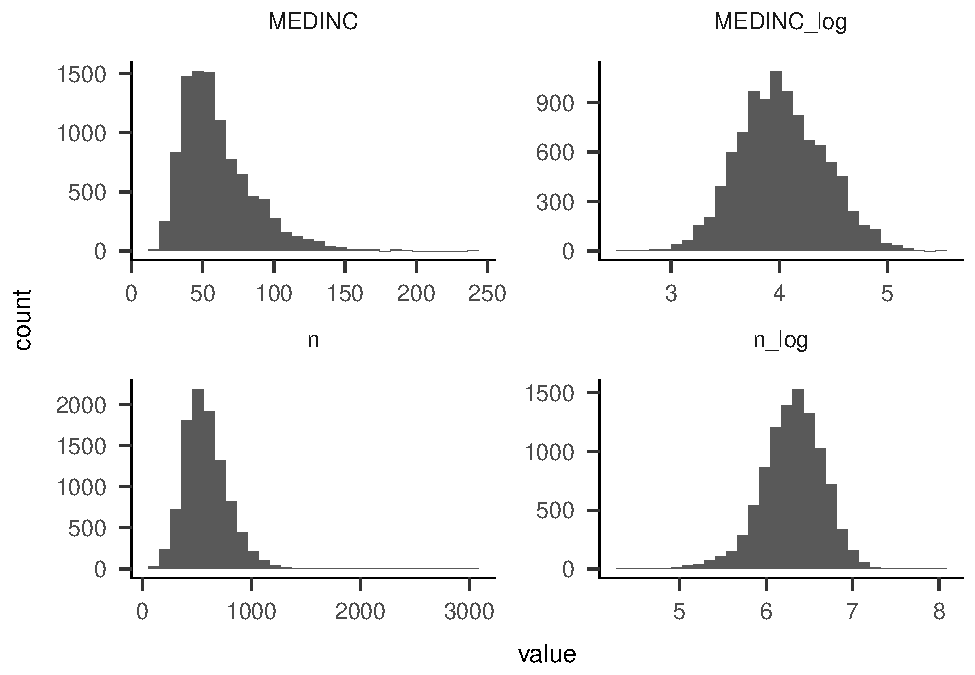
\includegraphics{Method_files/figure-latex/dists-1.pdf}
\caption{\label{fig:dists}Comparison of covariate distributions and their
log transformations.}
\end{figure}

\begin{figure}
\centering
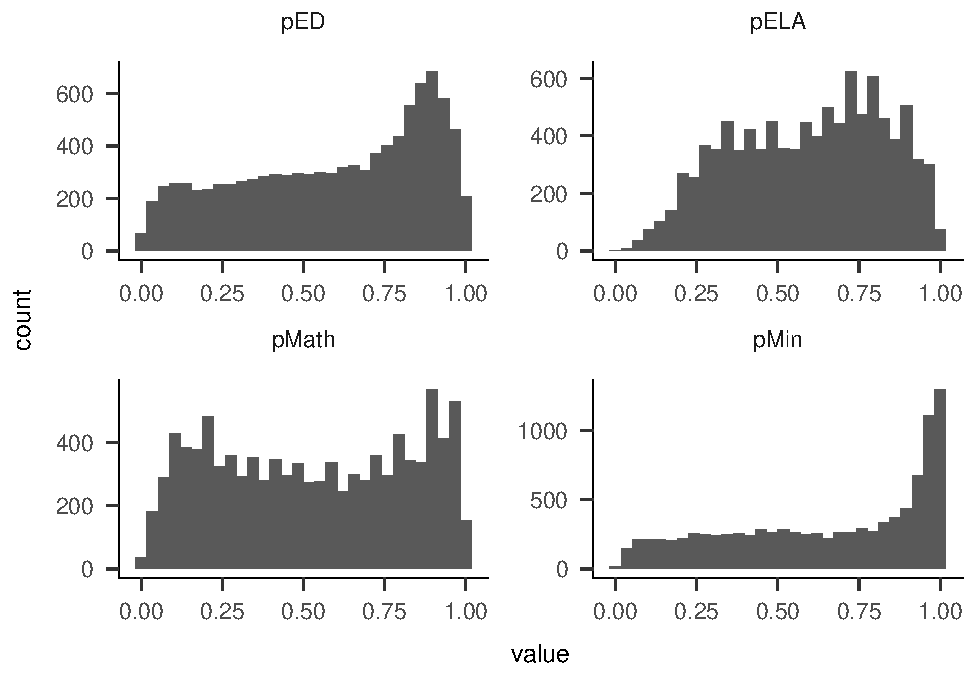
\includegraphics{Method_files/figure-latex/dists2-1.pdf}
\caption{\label{fig:dists2}Distributions of the remaining continuous
covariates.}
\end{figure}

\hypertarget{variable-transformations}{%
\subsubsection{Variable
Transformations}\label{variable-transformations}}

Log-transformation was used on school size (number of students) and
median income. This is done to allow proportional comparisons at the
extremes of the distributions (Hennig and Liao - 2013). For instance,
the difference between two schools with 4000 and 3000 students should be
weighed as much as the difference between two schools with 400 and 300
students when generating clusters. Figure \ref{fig:dists} displays a
comparison of the distribution of these variables and their logs. Figure
\ref{fig:dists2} displays the distribution of the remaining continuous
variables.

\hypertarget{subs}{%
\subsection{SUBS}\label{subs}}

Stratification using balanced sampling (SUBS) was performed prior to
simulation because the group of schools in each strata would be static
across conditions except where the balancing model is manipulated by
omitting median income. Per Tipton's (2013) original recommendation, we
use k-means clustering to partition the population into strata. This
requires selecting a distance metric, choosing the number of strata, and
performing the actual analysis.

\hypertarget{distance-metric}{%
\subsubsection{Distance Metric}\label{distance-metric}}

The set of covariates in both the full model (SUBS-F) and the omitted
variable model (SUBS-OV) include continuous covariates as well as binary
indicators for urbanicity (urban, suburban, and town/rural). Within this
context it is generally recommended to use Gower's (1971) general
dissimilarity distance (Everitt, 2011) which Tipton (2013) echos. This
method relies on different calculations of distance depending on the
type of covariates. Let \(d_{ii'h}\) be the distance between observed
values of covariate \(X_{h}\) for unit \(i\) and unit \(i'\) where
\(i \ne i'\). For categorical or dummy coded variables, \(d_{ii'h} = 1\)
if \(X_{ih} = X_{i'h}\) and \(d_{ii'h} = 0\) otherwise. For continuous
covariates, we use the following formula: \begin{align}
  d_{ii'h} = 1 - \frac{|X_{ih} - X_{i'h}|}{R_h}
\end{align} where \textbar{}.\textbar{} indicates absolute value,
\(X_{ih}\) and \(X_{i'h}\) are values of the \(h^{th}\) covariate for
units \(i\) and \(i'\), and \(R_h\) is the range of observations for
covariate \(X_h\). This method restricts the range of \(d_{ii'h}\) to
{[}0,1{]}. Finally, we calculate the general similarity between each
unit pair by taking the weighted average of the distances between all
covariates. Let \(d^{g}_{ii'}\) be the general similarity between unit
\(i\) and unit \(i'\) where \(i \ne i'\).

\begin{align}
  d^{g}_{ii'} = \frac{\sum^p_{h = 1}w_{ii'h}d_{ii'h}}{\sum^p_{h = 1}w_{ii'h}}
\end{align} where \(w_{ii'h} = 0\) if \(X_h\) is missing for either unit
and \(w_{ii'h} = 1\) otherwise. This produces an \(n\) by \(n\) distance
(or dissimilarity) matrix.

\hypertarget{number-of-clusters}{%
\subsubsection{Number of Clusters}\label{number-of-clusters}}

Selecting the number of clusters, \(k\), is one of the most difficult
problems in cluster analysis (Steinley, 2006). To date, the most
extensive investigation of methods for determining \(k\) was conducted
by Milligan and Cooper (1985) who analyzed 30 methods. However, aside
from the limited generalizability of this study, many methods are also
inappropriate in the context of non-hierarchical clustering and thus do
not support k-means clustering. Tipton (2013) states that both
statistical and practical criteria should be used in selecting the
number of clusters. Specifically, a large number of clusters would
result in more homogeneous strata and, in turn, a more robust sample.
However as strata become smaller they also become more difficult to
adequately sample from. Hennig and Liao (2013) also argue that the
method of selecting \(k\) should depend on the context of the clustering
and frame the issue as one of obtaining an appropriate
subject-matter-dependent definition of rather than a statistical
estimation. Ultimately three considerations were used to select the
number of clusters: the ratio of variability between clusters to the sum
of within and between cluster variability as recommended by Tipton
(2013), a generalized form of the Calinski-Harabasz index (Calinski and
Harabasz, 1974) proposed by Hennig and Liao (2013), and the practicality
of sampling from fewer clusters.

\begin{itemize}
\tightlist
\item
  Everitt (2011), p126

  \begin{itemize}
  \tightlist
  \item
    clusterSim
  \item
    Continuous data?

    \begin{itemize}
    \tightlist
    \item
      Calinski and Harabasz (1974)
    \item
      Duda and Hart (1973)
    \end{itemize}
  \item
    Steinley, D. (2006) K-means clustering: a half-century synthesis.
    British Journal of Mathematical \& Statistical Psychology, 59,
    1--34.
  \end{itemize}
\item
  Milligan and Cooper (1984)

  \begin{itemize}
  \tightlist
  \item
    list 30
  \end{itemize}
\item
  Sugar and James (2003) via Hennig \& Liao 2013 p 314

  \begin{itemize}
  \tightlist
  \item
    Modern look
  \end{itemize}
\end{itemize}

\hypertarget{cluster-analysis-1}{%
\subsubsection{Cluster Analysis}\label{cluster-analysis-1}}

Cluster analysis was performed using the \emph{cluster} package
(Maechler et. al.~2017) in R. First, the \emph{daisy} function is used
to compute an \(n\) by \(n\) pairwise distance matrix across all
observations. This function requires two parameters: (1) the data set,
and (2) the distance metric. For the full model, the data set included
the full list of school level covariates presented in table
\ref{tab:tbl-desc}. For the omitted variable model, median income was
omitted from the data set. For both models, the metric was set to
\enquote{gower}. Next the \emph{kmeans} function is used to generate
clusters. This method uses an optimization algorithm to classify units
into \(k\) clusters by minimizing the total within cluster sum of
squares. This function also requires two parameters: (1) the distance
matrix, and (2) the number of clusters to generate (\(k\)). For each
\(k\), it is recommended to run \emph{kmeans} at least 10 times, and
select the clustering that results in the smallest total within-cluster
sum of squares. {[}Get Citation{]}

Figure \ref{fig:ch-full} displays the Calinski-Harabasz (CH) index for
each \(k\) clusters generated for both the SUBS-F and SUBS-OV. The value
of \(k\) that maximizes the CH index should be selected. However we see
several local maxima: \(k = [2, 5, 8, 11]\) for SUBS-F, and
\(k = 2, 6, 10\) for SUBS-OV.

Taking the ratio of between-cluster SS to within-cluster SS and plotting
it against number of clusters creates a chart similar to an upside down
elbow graph. Figure \ref{fig:ratio-full} displays this for both SUBS-F
and SUBS-OV. Tipton (2013) recommends selecting the number of clusters
such that at least 80\% of the variability is between clusters,
indicated by the figure as a dashed line. Given this criteria it seems
that at least 10 clusters should be generated for SUBS-F, and 8 for
SUBS-OV. However we also see that after a sharp initial increase, the
slope of the graph begins to level out. This indicates that as we
increase the number of clusters, the benefit of doing so decreases,
while the difficulty of sampling from each cluster increases. In that
case after 6 or 7 clusters the difficulty of sampling may not be worth
such small increases in homogeneity within clusters.

Figure @ref(fig:k-size-full plots the sample size that needs to be
selected from each cluster to fulfill the proportional allocation
requirement such that the number of units sampled from each cluster is
proportional to the size of the cluster in the population. The dashed
line indicates the ideal allocation if all clusters were of equal size.
We see that for SUBS-F when 8 or less clusters are generated, they are
more equally sized, with the exception of 3 and 6 clusters where one is
much larger than the others. For SUBS-OV this is less apparent. Instead
a sensible cutoff may be determined by looking at the size of the
smallest cluster. At \(k > 7\) it seems that the smallest clusters would
require less than 5 units being sampled, which may be very difficult in
a practical setting.

In order to maintain comparability between methods, it was determined
that 6 clusters would be generated for both models, though in practice 7
clusters for the full model may be more prudent.

\begin{figure}
\centering
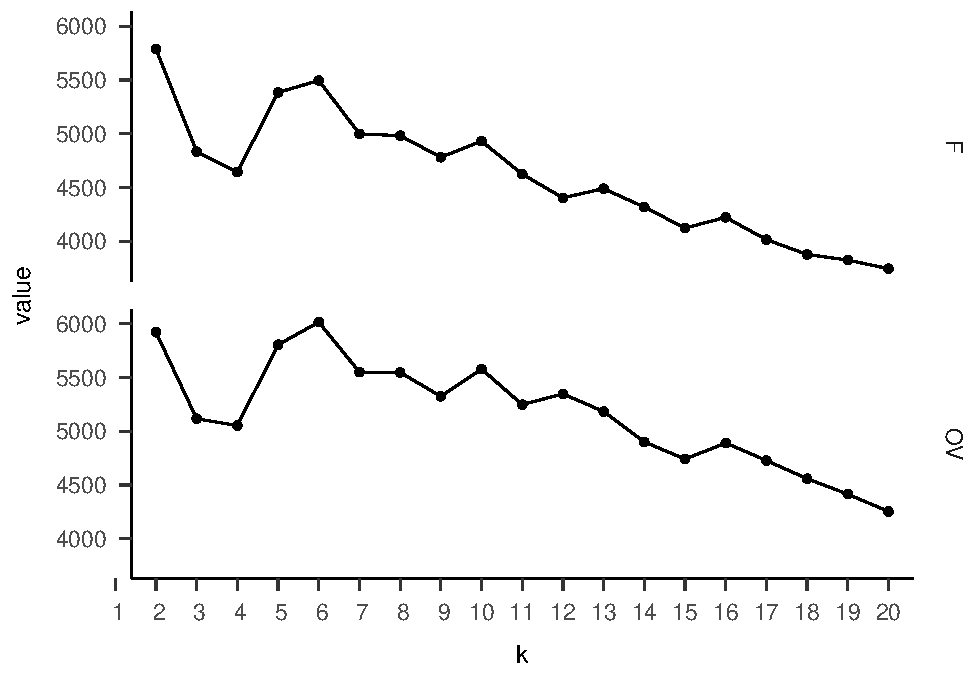
\includegraphics{Method_files/figure-latex/ch-full-1.pdf}
\caption{\label{fig:ch-full}Generalizd Calinski-Harabasz index}
\end{figure}

\begin{figure}
\centering
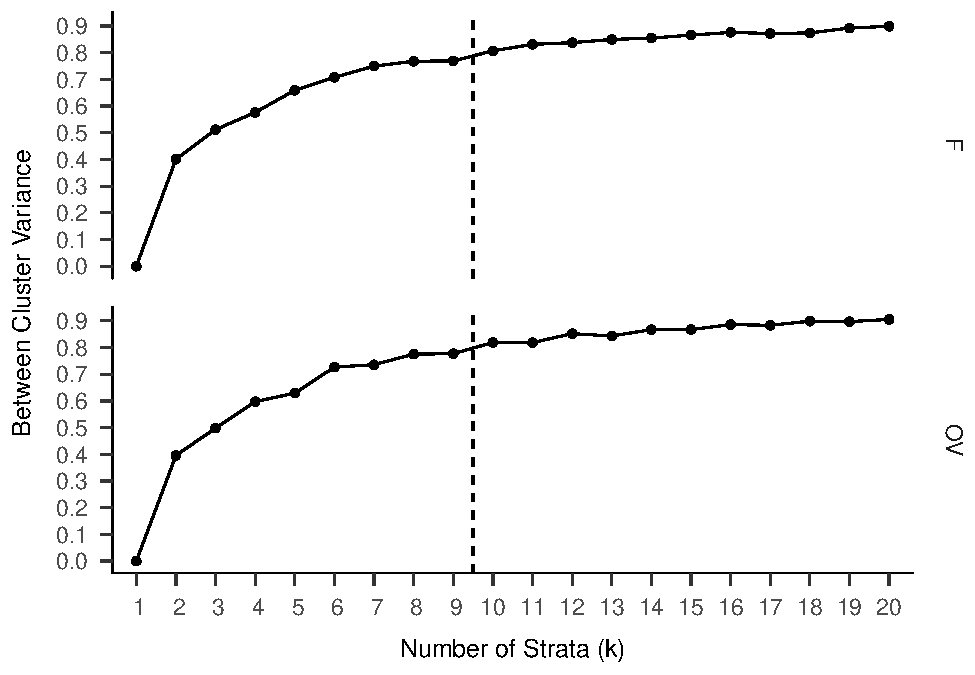
\includegraphics{Method_files/figure-latex/ratio-full-1.pdf}
\caption{\label{fig:ratio-full}Ratio of between cluster sum of squares to
total cluster sum of squares}
\end{figure}

\begin{figure}
\centering
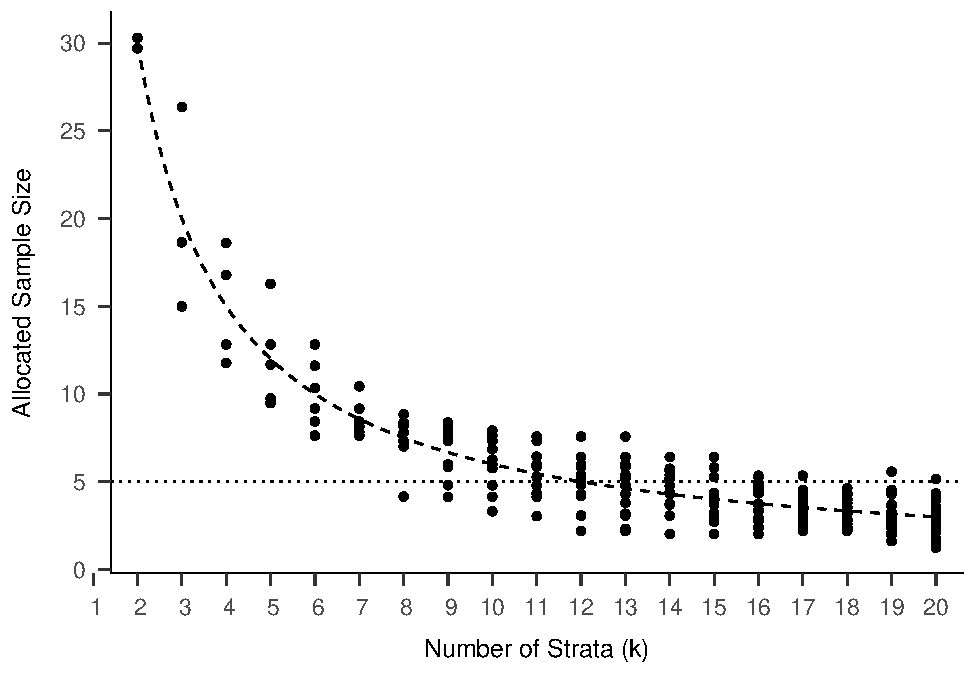
\includegraphics{Method_files/figure-latex/k-size-full-1.pdf}
\caption{\label{fig:k-size-full}Sampling requirements for each cluster}
\end{figure}

\newpage

\hypertarget{references}{%
\section{References}\label{references}}

\begingroup
\setlength{\parindent}{-0.5in}
\setlength{\leftskip}{0.5in}

\hypertarget{refs}{}

\endgroup


\end{document}
